\chapter{Extraktion von Bildmerkmalen}
\label{ch:merkmale}
Das Extrahieren von Bildmerkmalen ist zentraler Bestandteil aller Feature-based Algorithmen. Es muss festgelegt werden, welcher Typ von Merkmal gefunden werden soll, ein Suchalgorithmus ausgewählt werden und schlie{\ss}lich Überlegt werden durch welchen Deskriptor die Merkmale Beschrieben werden sollen.
%%%%%%%%%%%%%%%%%%%%%%%%%%%%%%%%%%%%%%%%%%%%%%%%%%%%%%%%%%%%%
\section{Auffinden von Merkmalen}
\subsection{Merkmale Beschreiben durch Nachbarschaftsoperationen}
% LINK SOURCE https://cmsc426.github.io/pano-prereq/
Merkmale sind lokale Punkte im Bild die durch die Pixel in ihrer Nachbarschaft charakterisiert sind. Gute Merkmale sind möglichst eindeutig bestimmbar und lassen sich nicht mit anderen Stellen im Bild verwechseln. Anwendungen wie Structure from Motion setzen Merkmale voraus, die sich auch nach Veränderungen des Bilds wie beispielsweise durch Translation, Rotation oder Lichtverhältnisse wiedererkennen lassen. Um diesen Anforderungen gerecht zu werden, eignen sich die Interest-Operatoren (auch Interest-Points, Corner).

Es sollen zunächst einige allgemeine Grundlagen zur Merkmalsdetektion betrachtet werden. Es wird einführend auf Kantendetektion eingegangen um von dort zu den Interest-Operatoren zu kommen.
\newline

Eine einfache Operation durch die Merkmale gefunden werden können, ist die Faltung.

\begin{equation}
  (f*g)(t) = \int_{-\infty}^{\infty} f(\tau)g(t-\tau)d\tau = \int_{-\infty}^{\infty} f(t-\tau)g(\tau)d\tau
  \label{eq:convolution}
\end{equation}

Dabei ist $g$ der Faltungskern (auch Kernel oder Filter) und bestimmt welche Operation auf das Bild angewandt wird. Durch den Kern kann ein Bild beispielsweise geglättet, schärfer gemacht werden oder Kanten extrahiert werden.

Faltunsgkerne lassen sich au{\ss}erdem als Approximation verwenden, wenn eine Ableitung des Bildes gebildet werden soll. Die Ableitung eines Bildes ist essentiell für die Bildverarbeitung, da sie den Gradient bildet. Durch die Bestimmung der Gradienten können Kanten und ihre Eigenschaften beschrieben werden. Der Gradientenvektor ist definiert als

\begin{equation}
  \nabla f=\left[\dfrac{\delta f}{\delta x}, \dfrac{\delta f}{\delta y}\right]
\end{equation}

Der Gradient eines Bildes zeigt in die Richtung, in der es die grö{\ss}te Veränderung der Intensitätswerte der Pixel gab. Daher lässt sich die Richtung der grö{\ss}ten Veränderung bestimmen durch

\begin{equation}
  \theta=tan^{-1}\left(\dfrac{\delta f}{\delta y}\Bigg{/}\dfrac{\delta f}{\delta x}\right)
\end{equation}

Die Richtung verläuft immer Senkrecht zur Kante. Die Stärke des Anstiegs und damit die Stärke der Kante und ist gegeben durch den Betrag des Gradienten

\begin{equation}
  ||\nabla f|| = \sqrt{\left(\dfrac{\delta f}{\delta x}\right)^2 +
  \left(\dfrac{\delta f}{\delta y}\right)^2}
\end{equation}

Für die Bildverarbeitung können die Partiellen Ableitungen praktisch berechnet werden als 

\begin{equation}
  \begin{split}
  \delta x &= f(x+1,y) -  f(x,y)\\
  \delta y &= f(x,y+1) -  f(x,y)
  \end{split}
\end{equation}

Beispiele für bekannte Kanten Operatoren sind der Sobel Operatior, Prewitt, Roberts, Laplacian of Gaussian (LoG) und Canny.

\begin{equation}
  \rho(\tau)= K\int_{-\infty}^\infty x(t) m(t + \tau) {\rm d}t
\end{equation}
Die gesuchten Interest-Operatoren entstehen durch das aufeinandertreffen zweier Kanten. Das bedeutet in der Nachbarschaft dieses Punktes existieren zwei starke und unterschiedliche Gradientenanstiege. Die einfachste Art Interest-Points zu detektieren ist durch Korrelation.

\subsection{Algorithmen zum Auffinden von Interest-Operatoren}
Für die Lokalisierung werden Detektoren verwendet, die nach Interest-Operatoren im Bild suchen. Interest-Punkte haben gegenüber Punkten und Kanten die entscheidende Eigenschaft invariant gegenüber Veränderungen in Rotation, Skalierung und Lichtverhältnissen zu sein.
 
\subsubsection{Moravec-Operator}
Der Moravec-Operator wurde 1977 veröffentlicht. Berechnet die mittlere quadratische Gradientensumme und bestimmt Ecken anhand eines Schwellwertes. Der Moravec-Operator eignet sich nicht im Kontext von Lokalisierung, da er nicht Rotationsinvariant ist.

\subsubsection{Harris Corner Detektor}
\begin{figure}[!h]
  \centering
    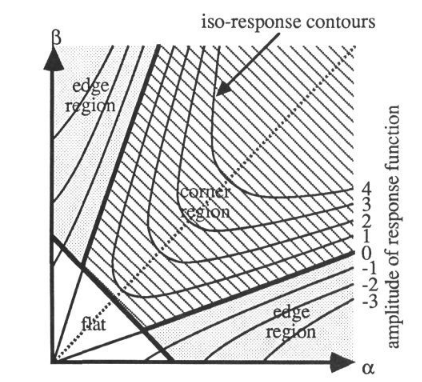
\includegraphics[width=0.4\linewidth]{harris_autocorrelation.png}
    \caption[Harris Interest-Operator Detektor]{Klassifikation der Autokorrelation in Edge, Flat und Corner Region. $\alpha$  und $\beta$ entsprechen $\lambda_1$ und $\lambda_2$ (Harris, 1988 \cite{Harris88alvey.Ha})}
\end{figure} 

Der Harris Corner Detektor wurde 1988 basierend auf dem Moravec-Operator veröffentlicht. Der wesentliche Unterschied ist, dass Harris eine Rotations- und Skalierungsinvarianz durch integration von Autokorrelation erreicht. 
Auf einen Bildpunkt angewandt kann durch eine Funktion $E(u,v)$ die Veränderung der Intensitätswerte für eine Verschiebung eine Punktes in jede Richtungen gefunden werden.

% Windows Funktion: Box oder Gaussian
\begin{equ}[!ht]
  \begin{equation}
    E(u,v) = \sum_{x,y} \underbrace{w(x,y)}_{\text{Window Fkt}} [\underbrace{[I(x+u, y+v)}_{\text{verschobene Intensität}} - \underbrace{I(x,y) ]^2}_{\text{Original Intensität}}
  \end{equation}
  \caption{Formel des Harris-Corner Detektors}
\end{equ}

Für die Detektion von Interest-Operatoren muss die Funktion maximiert werden.
Verwendung der Taylor Approximation 1. Grades führt zu nachfolgenden Schritten. 

%
\begin{equation}[!ht]
  f(x+u, y+v) \approx f(x,y) + uf_{x}(x,y) + vf_{y}(x,y)
\end{equation}
\begin{equation}
  \begin{aligned}
    E(u,v) &= \sum \left[ I(x+u, y+v) - I(x,y) \right]^2 \\
    &= \sum \left[ I(x,y) + uI_{x} + vI_{y} - I(x,y) \right]^2 \\
    &= \sum u^2I_{x}^2 + 2uvI_{x}I_{y}-v^2I_y^2\\
    &= \sum \begin{bmatrix} u & v \end{bmatrix} 
    \begin{bmatrix} I_x^2 & I_xI_y \\ I_xI_y & I_y^2 \end{bmatrix} 
    \begin{bmatrix}u \\v \end{bmatrix} \\
    &= \begin{bmatrix} u & v \end{bmatrix} \left(\sum 
    \begin{bmatrix} I_x^2 & I_xI_y \\ I_xI_y & I_y^2 \end{bmatrix} 
    \right) \begin{bmatrix}u \\v \end{bmatrix} 
  \end{aligned}
\end{equation}

Für kleine Verschiebungen ergibt sich die bilineare Approximation

\begin{equation}
  E(u,v) \cong \begin{bmatrix}
    u,v
  \end{bmatrix} M \begin{bmatrix}
    u\\ v
  \end{bmatrix}
\end{equation}

Mit M als

\begin{equation}
  M = \sum_{x,y} w(x,y)  
  \begin{bmatrix} I_x^2 & I_xI_y \\ I_xI_y & I_y^2 \end{bmatrix}  
\end{equation}

Der zweite Part des Harris Operators ist die Score Funktion.

\begin{equation}
  R = \lambda_1 \lambda_2 - k(\lambda_1 + \lambda_2)^2 = \det(M) - k(\operatorname{trace}(M))^2
\end{equation}

Durch den Score wird überprüft, ob das Fenster einen Interest-Operator enthält. 

\subsubsection{Shi-Tomasi Detektor (GFFT)}
\begin{figure}[!ht]
  \centering
  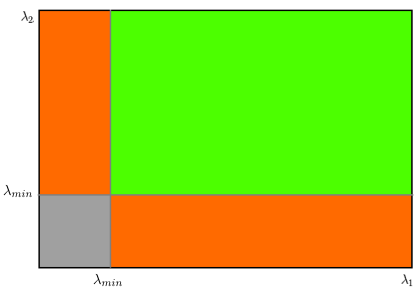
\includegraphics[width=0.45\textwidth]{pictures/03_shitomasi_space.png}
  \caption[GFTT Detektor Merkmalsfindung]{Ein Merkmal wird bei GFTT durch eine Min-Funktion bestimmt. Nur wenn $\lambda_1$ und $\lambda_2$ über dem Grenzwert $\lambda_{min}$ liegen, handelt es sich um einen Interest-Operator (grüner Bereich) (OpenCV Docs GFTT, 2022)}
\end{figure}

Das erste mal würde dieser Detektor 1994 unter dem Titel \textit{Good Features To Track} in einem Paper veröffentlicht. Daher wird er sowohl als Shi-Tomasi als auch GFTT Detektor bezeichnet. Dieser Detektor ist gleich dem Harris Detektor mit Ausnahme einer Änderung im Scoring. Statt das Scoring über die Eigenwerten zu berechnen, wurde vorgeschlagen, die Score direkt aus einer Min-Funktion der Eigenwerte zu setzen. 

\begin{equation}
  R = min(\lambda_1,\lambda_2)
\end{equation}

Dadurch kann die Ursprünglich eingeführte Funktion weggelassen werden.

\subsubsection{FAST}
Features from Accelerated Segment Test (FAST) wurde 2006 veröffentlicht. FAST ist für seine Geschwindigkeit bekannt. Anwendungen wie SLAM haben sehr hohe Anforderungen an die Laufzeit der Merkmalsdetektoren. FAST hat eine kürzere Rechenzeit als die vorangegangenen Detektoren und wurde speziell für den Einsatz in zeitkritischen Anwendungen entwickelt.

\begin{figure}[!ht]
  \centering
  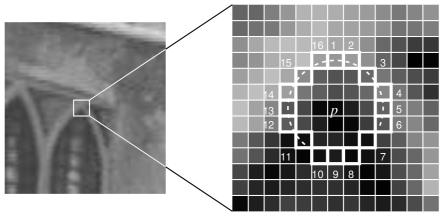
\includegraphics[width=0.75\textwidth]{pictures/03_fast_speedtest.jpg}
  \caption[FAST Detektor Speedtest]{FAST Detektor Performance Test, (E. Rosten and R. Porter and T. Drummond, 2010 \cite{FAST})}
\end{figure}

FAST legt einen Kreis von 16 Pixel um ein interessantes Pixel q. Der Kreis wird durchnummeriert und der Intensitätswert $Iq$ von q erfasst. Es wird Verglichen ob im Kreis N zusammenhängende Pixel heller als $I_q+thresh$ oder dunkler als $I_q-tresh$ sind. Wobei $thresh$ ein Grenzwert ist.\newline

Nun werden nicht alle 16 Pixel untersucht. FAST schlägt einen High-Speed-Test vor bei dem nur 4 Pixel getestet werden. Zuerst werden die Intensitäten von 1 und 9 gegen den Grenzwert getestet, dann 5 und 13. Ist p ein Interest-Punkt müssen mindestens 3 dieser Pixel heller as $I_q + thresh$ oder dunkler als $I_q - tresh$ sein.\newline

Das Verfahren ist tatsächlich sehr schnell, wei{\ss}t aber einige Mängel auf. Die Empfehlung ist eine Kombination mit einem Machine Learning Ansatz, dadurch können die Nachteile gut behoben werden. \cite{cvdocFAST} Für den Systementwurf wurden generell nur direkte Verfahren ohne Machine Learning ausgewählt und anstatt des FAST Detektors daher der GFTT (Shi-Tomasi Detektor) Detektor eingesetzt.


%
\pagebreak
%%%%%%%%%%%%%%%%%%%%%%%%%%%%%%%%%%%%%%%%%%%%%%%%%%%%%%%%%%%%%
\section{Matching}
Beim Feature Matching wird festgestellt, ob es sich bei Merkmalen die in zwei verschiedenen Bildern gefunden wurden um das selbe Merkmal handelt. Hierzu wird für jedes Merkmal des ersten Bildes in dessen ursprünglichen Position im zweiten Bild gesucht. Wie gro{\ss} die Suchumgebung um die ursprüngliche Position herum ist, hängt von der gewählten Abstandsmetrik des Suchalgorithmus ab.
\newline

Generell hängt die Leistung der Matchingverfahren von den Eigenschaften der zugrunde liegenden Merkmale als auch von der Wahl der zugeordneten Bilddeskriptoren ab. Es ist daher wichtig die geeigneten Detektoren und Deskriptoren auszuwählen. Beispielsweise wäre für ein Mikroskop Bild einer organischen Struktur ein Blob-Detektor wahrscheinlich am besten geeignet, währen in einer Urbanen Umgebung mit menschengemachten, geometrischen Strukturen ein Interest-Operator wesentlich erfolgversprechender ist.
\newline

\subsection{Übereinstimmungen finden}
Zwischen zwei Bildern sollen gemeinsame Merkmale gefunden werden. Aus gefundenen Merkmalen besitzt jedes Bild eine eigene Menge von Merkmalsdeskriptoren. Jeder Deskriptor befindet sich an einer bestimmten Stelle im Bild. Für das Matching wird ein Deskriptor des ersten Bildes nicht mit der gesamten Menge an Deskriptoren des zweiten Bildes verglichen. Stattdessen wird um die Position, an der sich der Deskriptors im ersten Bild befindet, eine Region of Interest bzw Suchfenster gebildet. Es werden dann nur Deskriptoren des zweiten Bildes für den Abgleich herangezogen, die innerhalb dieser Region auftreten. Selbst beim, von OpenCV implementierten, Brute Force Matching wird in einem bestimmten Abstand zum gesuchten Deskriptor gesucht. 

\begin{equation}
    \begin{aligned}
      d_{euclidean}(p,q) & = \Vert q-p {\Vert}_2&\\
      & = \sqrt{(q_1 - p_1)^2 + ... + (q_n - p_n)^2}&\\
      & = \sqrt{\sum_{i = 1}^{n} (q_i - p_i)^2  } 
      \label{eq:l2norm}
    \end{aligned}
\end{equation}

Die Grö{\ss}e des Suchfensters wird über den Abstand angegeben. Bei klassischen Deskriptoren wie SIFT und SURF wird im Euklidischen Abstand gesucht. Bei Binär-Deskriptoren wie ORB und BRISK sollte der Hamming-Abstand verwendet werden.   

\begin{equation}
  d_{hamming} \left ( q,p \right ) = \sum_{i=0}^{n-1} \left ( q_i \oplus p_i \right )
  \label{eq:hamming}
\end{equation}

Dei Begründung liegt in der unterschiedlichen Beschaffenheit der Deskriptoren. Bei SIFT repräsentieren sie Histogramme von gerichteten Gradienten. Bei ORB handelt es sich um Binärwörter die durch den XOR-Operator verglichen werden können wie in Gleichung \ref{eq:hamming} zu sehen. 

\subsection{Matching Ergebnisse Filtern}
Die Matches die durch die Suche bestimmt wurden sind teilweise nur sich stark ähnelnde Merkmale und keine echten Übereinstimmungen. Die Ergebnisse sind also von unterschiedlicher Qualität. Sie müssen daher noch gefiltert werden. Zum einen wird so bei den folge Schritten Zeit gespart. Zum anderen handelt es sich im Grunde um Ausrei{\ss}ern die ohne Filterung zu Fehlern in nachfolgenden Schätzungen führen werden.

Um die Ergebnisse zu Filtern gibt es drei Unterschiedliche Ansätze:

\begin{description}
  \item[Lowes Distance Ratio Test] Der Test überprüft ob es in der direkten Nachbarschaft, weitere Matches gibt. Falls ja und das Match hat einen Ratio nahe eins, sind das Match und sein Nachbar von gleicher Qualität. Bei dem Ausgewählten Match handelt es sich dann mit 50\% Wahrscheinlichkeit um einen Ausrei{\ss}er. Daher werden beide Matches verworfen. Der Ratio unter dem die Merkmale liegen müssen ist variabel und wird über einen threshold and die Funktion übergeben. \cite{Lowe04distinctiveimage} 
  \item[Cross Check] Beim Cross-Check werden die Resultate der beiden Bilder darauf Verglichen, ob das beste Match in Set A auch das beste Match in Set B war und umgekehrt. Cross Checking kann beim Brute Force Matcher verwendet werden. 
  \item[Geometrischer Test] Ausgleichsverfahren basierend auf der Methode der kleinsten Quadrate wie beispielsweise RANSAC. 
\end{description}

\subsection{Stereo Matching}
Der Abgleich von Stereokamera Bildpaaren unterscheidet sich vom Matching in normalen Bildsequenzen. Stereo Bildpaare wurden zum gleichen Zeitpunkt aufgenommen und sind so ausgerichtet, dass sich die Merkmale bei beiden Bildern in der gleichen Reihe befinden.

Prinzipiell wird beim Stereo Matching für jedes Pixel wie folgt vorgegangen:

Zuerst wird die Epipolarlinie gesucht. 

Anschlie{\ss}end wird die Linie nach der besten Übereinstimmung abgesucht.

Schlie{\ss}lich wird die Tiefe aus der Verschiebung berechnet

\begin{equation}
  Z = \frac{bf}{d}
  \label{eq:depth}
\end{equation}

\subsection{Semi Global Block Matching}
Beim Stereo Block Matching wird nicht pixelweise verglichen, sondern kleine Regionen. Ein Fenster wird die Epipolarlinie des rechten Bildes entlang geschoben und der Inhalt mit der Ausgewählten Region im linken Bild verglichen.
\begin{figure}[!ht]
  \centering
  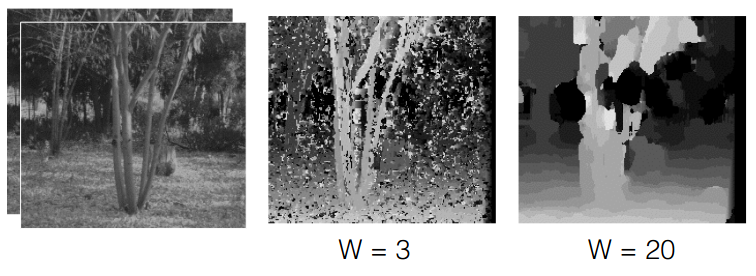
\includegraphics[width=0.85\textwidth]{pictures/03_windowsize.png}
  \caption[Effekt der Fenstergö{\ss}e bei Disparitätenkarten]{Effekt der Fenstergrö{\ss}e, (Kris Kitani - Carnegie Mellon University, 2020)}
\end{figure}

Die Fenstergrö{\ss}e wirkt sich direkt auf die Disparitätenkarte aus. Sie beschreibt die Verschiebung zwischen den beiden Bildern und enthält noch nicht die gesamte Tiefeninformation. Tiefe wird mit Hilfe der Disparität berechnet, wie gezeigt in Gl. \ref{eq:depth}. Für kleine Fenstergrö{\ss}en enthält die Disparitätenkarte mehr Details aber auch mehr Rauschen. Für gro{\ss}e Fenster ist die Karte glatter und hat weniger Details.

Generell beschleunigt Block Matching die Erstellung der Disparitätenkarte da weniger Vergleiche vorgenommen werden müssen. In Regionen ohne Texturen oder bei Bildern in denen sich Muster oft wiederholen kann das Verfahren fehlschlagen. Teile der Karte sind dann Schwarz und ohne Information. 

\section{Deskriptoren}
Für gefundene Merkmale werden Deskriptoren berechnen. Sie sind sozusagen der Fingerabdruck von jedem Merkmal. Mithilfe des Deskriptors sollen Merkmale eindeutig und zuverlässig wiedererkannt werden können. Vor allem auch dann, wenn sich die Abgebildete Szene zwischen zwei Bildern verändert hat. Ein Interest-Operator bleibt als solcher erkennbar, auch wenn die Region gedreht wird. Schwieriger verhält es sich mit der Skalierung. 
\newline

Mit dem Harris-Detektor können bei einer gro{\ss}en Änderung der Skalierung der Interest-Punkt nicht mehr wiedergefunden werden. Die ersten skalierungsinvarianten Detektoren kamen mit SURF (2006) und SIFT (1999). SIFT (Scale-Invariant Feature Transform) liefert sehr gut Resultate in Verbindung mit Lokalisierungsaufgaben. Allerdings braucht der Deskriptor viel Rechenleistung und ist zu langsam für Echtzeitanforderungen. ORB ist eine weit verbreitete, wesentlich weniger Rechenaufwendige Alternative. Für den Systementwurf wurden zu Beginn beide Algorithmen betrachtet. Zusammen mit der Simulationsumgebung verbrauchten die Visuelle Odometrie SOftware mit SURF zu viele Ressourcen. Der Wechsel zu ORB brachte eine wesentliche Entlastung der CPU.
\newline 

Diese Beobachtung lässt sich einfach durch eine Kategorisierung der Berechnungsmethoden der Algorithmen erklären.

SIFT gehört zu der Klasse der \textit{Histogram of Oriented Gradients} (HOG) Deskriptoren währen ORB zu den \textit{Binären} Deskriptoren zählt. Ein Deskriptor hat immer eine Beschreibung für einen interessanten Pixel und seiner unmittelbare Nachbarschaft  sowie eine Distanzfunktion mit der die Ähnlichkeit zwischen zwei Deskriptoren (des gleichen Typs) bestimmt wird.

\subsection{Histogram Deskriptoren}
\begin{figure}[!ht]
  \centering
  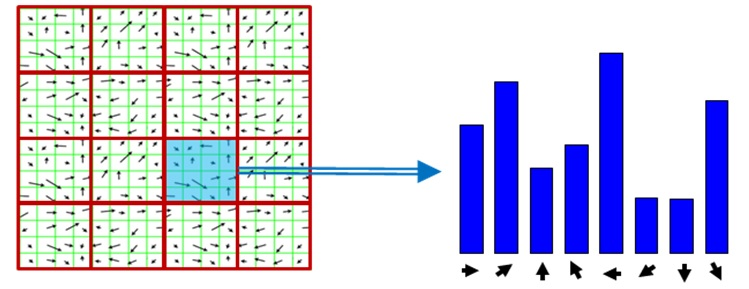
\includegraphics[width=0.75\textwidth]{03_HOG_01.jpg}
  \caption[Histogram Deskriptor aus Gradienten]{Berechnen der Histogramme für die Ausrichtung der Gradienten (Lowe, 1999 \cite{SIFT})}
\end{figure}

Histograms of Oriented Gradients (HOF) Deskriptoren die in der Praxis häufig eingesetzt werden sind SIFT \cite{SIFT} und SURF\cite{SURF}. Im folgenden werden die Rechenschritte für SIFT beispielhaft erläutert.
\newline

Bei dieser Art von Deskriptor wird ein Region um das Merkmal, beispielsweise 16x16 Pixel, genommen. Die Region wird wiederum in kleinere Subregionen unterteilt, beispielsweise 4x4. Für alle Pixel wird die Orientierung berechnet und anschlie{\ss}end der Gradient für die Subregion. Daraufhin kann ein Histogram für die Subregionen erstellt werden.

Durch Aneinanderreihen der Histogramme ergibt sich ein Merkmalsvektor. Für das Beispiel waren es 16 Subregionen mit 8 Histogrammen per Subregion, also ein Merkmalsvektor der mit 128 (16*8) Elementen. 

\subsection{Binäre Deskriptoren}

\begin{figure}[!ht]
  \centering
  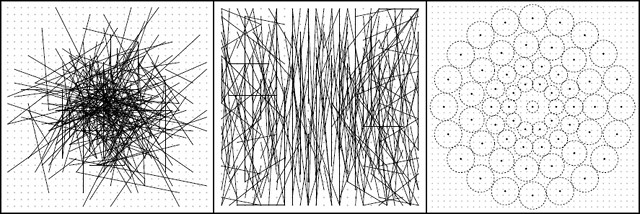
\includegraphics[width=\textwidth]{03_brief_orb_brisk_640.jpg}
  \caption[Muster binärer Deskriptoren]{Deskriptor Muster, von Links nach Rechts: BRIEF, ORB, BRISK. (Heinly, 2012 \cite{binDesc})}
\end{figure}

Anstatt, wie bei HOG Deskriptoren, die Gradienten aller Pixel zu berechnen, werden bei binären Deskriptoren Intensitätswerte verglichen. Das Ergebnis des Vergleichs sind Binärwörter. Diese können direkt durch den XOR-Operator abgeglichen werden, was das Matching deutlich beschleunigt. 

Beispiele für bekannte binäre Deskriptoren sind BRIEF \cite{BRIEF}, ORB \cite{ORB} und BRISK\cite{BRISK}. Binärdeskriptoren können anhand von drei Attributen verglichen werden.

\begin{description}
  \item[Das Abtastmuster] Ein Muster das auf die Region um den Deskriptor gelegt wird. Es werden nur Punkte die auf dem Muster liegen untersucht.
  \item[Ausrichtungskompensation] Eine Methode um die Orientierung des Merkmals zum bestimmen und es zu drehen um Rotation des Merkmals zwischen den Bildern auszugleichen.
  \item[Stichprobenpaare] Auswahl von Punkten die Verglichen wurden welche im Binärwort eingetragen werden sollen. 
\end{description}

Es müssen nicht alle diese Attribute in binären Deskriptor vorhanden sein, sie helfen lediglich bei der Klassifizierung. Wie auch zuvor bei HOG Deskriptoren wird eine Region ausgewählt. Auf die Region wird ein Muster gelegt. Je nach Einstellung werden N Punktpaar auf dem Muster ausgewählt und deren Intensitätswerte verglichen. Ist Punkt A heller als Punkt B ist das Resultat eine 1, sonst 0. Dies wird für die N Punktpaare wiederholt. Anschlie{\ss}end wird ein Strichprobenmenge aus N entnommen und als Binärwort abgelegt. Für das spätere Matching mit einem anderen Deskriptor muss lediglich die Summe über die XOR Verknüpften Binärwörter gebildet werden um die Ähnlichkeit zu bestimmen. Sum(xor(string1, string2)) ist die sog. Abstandsfunktion. Aus der Abstandsfunktion lässt sich schlie{\ss}en, das die Reihenfolge der gespeicherten Werte keine Rolle spielt.


\subsection{ORB - Oriented FAST and Rotated BRIEF}
ORB ist eine Erweiterung des FAST Detektors und BRIEF Deskriptors. BRIEF war 2011 der erste veröffentlichte binäre Deskriptor. Er hat noch kein festes Muster. Stattdessen wird ein zufälliges Muster erstellt. Der Deskriptor erzielt damit eine hohe Wiedererkennungsrate, solange es keine Rotation im Bild gibt, denn es wurde auch noch keine Ausrichtungskompensation implementiert. ORB erweitert BRIEF mit einer entsprechenden Methode und ist damit rotationsinvariant.
Um die Orientierung eines Interest-Operators zu messen verwendet ORB einen \textit{intensity centroid} \cite{Rosin1999MeasuringCP}, bestimmt also den Schwerpunkt der Intensitätswerte. Die Momente der Region errechnen sich zu
\begin{equation}
  \centering
  m_{pq}=\underset{x,y}{\Sigma}x^py^qI(x,y)
\end{equation}
mit I(x,y) als Intensitätsfunktion und p,q als Grad des Moments. Der Schwerpunkt wird berechnet durch
\begin{equation}
  \centering
  C = ( \frac{m_{10}}{m_{00}}, \frac{m_{01}}{m_{00}})
\end{equation}
und schlie{\ss}lich die Richtung durch 
\begin{equation}
  \centering
  \theta = atan2(m_{01}m_{10})
\end{equation}
